\begin{center}

\includegraphics[width=0.6\textwidth]{content/3/chapter6/images/7.png}\\
Cippi studies the atomics
\end{center}

Atomics receives a few important extensions in C++20. Probably the most important ones are atomic references and atomic smart pointers.

\subsubsubsection{6.2.1\hspace{0.2cm} std::atomic\_ref}

The class template std::atomic\_ref applies atomic operations to the referenced object.

Concurrent writing and reading of an atomic object ensures that there is no data race. The lifetime of the referenced object must exceed the lifetime of the atomic\_ref. When any atomic\_ref is accessing an object, all other accesses to the object must use an atomic\_ref. In addition, no subobject of the atomic\_ref-accessed object may be accessed by another atomic\_ref.

\hspace*{\fill} \\ %插入空行
\noindent
\textbf{6.2.1.1\hspace{0.2cm} Motivation}

Stop. You may think that using a reference inside an atomic would do the job. Unfortunately not.

In the following program, I have a class ExpensiveToCopy, which includes a counter. The counter is concurrently incremented by a few threads. Consequently, counter has to be protected.

\hspace*{\fill} \\ %插入空行
\noindent
Using an atomic reference
\begin{lstlisting}[style=styleCXX]
// atomicReference.cpp

#include <atomic>
#include <iostream>
#include <random>
#include <thread>
#include <vector>

struct ExpensiveToCopy {
	int counter{};
};

int getRandom(int begin, int end) {
	
	std::random_device seed; // initial seed
	std::mt19937 engine(seed()); // generator
	std::uniform_int_distribution<> uniformDist(begin, end);
	
	return uniformDist(engine);
}

void count(ExpensiveToCopy& exp) {

	std::vector<std::thread> v;
	std::atomic<int> counter{exp.counter};
	
	for (int n = 0; n < 10; ++n) {
		v.emplace_back([&counter] {
			auto randomNumber = getRandom(100, 200);
			for (int i = 0; i < randomNumber; ++i) { ++counter; }
		});
	}
	
	for (auto& t : v) t.join();

}

int main() {
	
	std::cout << '\n';
	
	ExpensiveToCopy exp;
	count(exp);
	std::cout << "exp.counter: " << exp.counter << '\n';
	
	std::cout << '\n';

}
\end{lstlisting}

Variable exp (line 42) is the expensive-to-copy object. For performance reasons, the function count (line 22) takes exp by reference. Function count initializes the std::atomic<int> with exp.counter (line 25). The following lines create 10 threads (line 27), each performing the lambda expression, which takes counter by reference. The lambda expression gets a random number between 100 and 200 (line 29) and increments the counter exactly as often. The function getRandom (line 13) starts with an initial seed and creates via the random-number generator \href{https://en.wikipedia.org/wiki/Mersenne_Twister}{Mersenne Twister} a uniform distributed number between 100 and 200.

In the end, the exp.counter (line 44) should have an approximate value of 1500 because ten threads increment on average 150 times. Executing the program on the \href{https://wandbox.org/}{Wandbox online compiler} gives me a surprising result.

\begin{center}
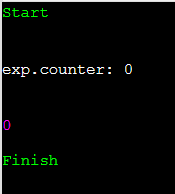
\includegraphics[width=0.4\textwidth]{content/3/chapter6/images/8.png}\\
Surprise with an atomic reference
\end{center}

The counter is 0. What is happening? The issue is in line 25. The initialization in the expression std::atomic<int> counter{exp.counter} creates a copy. The following small program exemplifies the issue.

\hspace*{\fill} \\ %插入空行
\noindent
Copying the reference
\begin{lstlisting}[style=styleCXX]
// atomicRefCopy.cpp

#include <atomic>
#include <iostream>

int main() {

	std::cout << '\n';
	
	int val{5};
	int& ref = val;
	std::atomic<int> atomicRef(ref);
	++atomicRef;
	std::cout << "ref: " << ref << '\n';
	std::cout << "atomicRef.load(): " << atomicRef.load() << '\n';
	
	std::cout << '\n';

}
\end{lstlisting}

The increment operation in line 13 does not address the reference ref (line 11). The value of ref is not changed.

\begin{center}
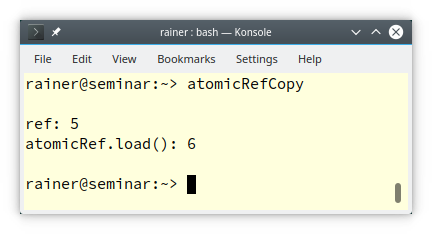
\includegraphics[width=0.4\textwidth]{content/3/chapter6/images/9.png}\\
Copying the reference
\end{center}

Replacing the std::atomic<int> with std::atomic\_ref<int> solves the issue.

\hspace*{\fill} \\ %插入空行
\noindent
Using a std::atomic\_ref
\begin{lstlisting}[style=styleCXX]
// atomicRef.cpp

#include <atomic>
#include <iostream>
#include <random>
#include <thread>
#include <vector>

struct ExpensiveToCopy {
	int counter{};
};

int getRandom(int begin, int end) {
	std::random_device seed; // initial randomness
	std::mt19937 engine(seed()); // generator
	std::uniform_int_distribution<> uniformDist(begin, end);
	
	return uniformDist(engine);
}

void count(ExpensiveToCopy& exp) {
	
	std::vector<std::thread> v;
	std::atomic_ref<int> counter{exp.counter};
	
	for (int n = 0; n < 10; ++n) {
		v.emplace_back([&counter] {
			auto randomNumber = getRandom(100, 200);
			for (int i = 0; i < randomNumber; ++i) { ++counter; }
		});
	}

	for (auto& t : v) t.join();
}

int main() {
	
	std::cout << '\n';
	
	ExpensiveToCopy exp;
	count(exp);
	std::cout << "exp.counter: " << exp.counter << '\n';
	
	std::cout << '\n';
}
\end{lstlisting}

Now, the value of counter is as expected:

\begin{center}
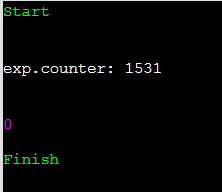
\includegraphics[width=0.4\textwidth]{content/3/chapter6/images/10.png}\\
The expected result with std::atomic\_ref
\end{center}

In keeping with \href{https://en.cppreference.com/w/cpp/atomic/atomic}{std::atomic}, type std::atomic\_ref can be specialized and supports specializations for the built-in data types.

\hspace*{\fill} \\ %插入空行
\noindent
\textbf{6.2.1.2\hspace{0.2cm} Specializations of std::atomic\_ref}

You can specialize std::atomic\_ref for user-defined types, use partial specializations for pointer types, or full specializations for arithmetic types such as integral or floating-point types.

\hspace*{\fill} \\ %插入空行
\noindent
\textbf{6.2.1.2.1\hspace{0.2cm} Primary Template}

The primary template std::atomic\_ref can be instantiated with a \href{https://en.cppreference.com/w/cpp/types/is_trivially_copyable}{TriviallyCopyable} type T.

\begin{lstlisting}[style=styleCXX]
struct Counters {
	int a;
	int b;
};

Counter counter;
std::atomic_ref<Counters> cnt(counter);
\end{lstlisting}

\hspace*{\fill} \\ %插入空行
\noindent
\textbf{6.2.1.2.2\hspace{0.2cm} Partial Specializations for Pointer Types}

The standard provides partial specializations for a pointer type: std::atomic\_ref<T*>.

\hspace*{\fill} \\ %插入空行
\noindent
\textbf{6.2.1.2.3\hspace{0.2cm} Specializations for Arithmetic Types}

The standard provides specialization for the integral and floating-point types: std::atomic\_ref<arithmetic type>.

\begin{itemize}
\item 
Character types: char, char8\_t (C++20), char16\_t, char32\_t, and wchar\_t

\item 
Standard signed-integer types: signed char, short, int, long, and long long

\item 
Standard unsigned-integer types: unsigned char, unsigned short, unsigned int, unsigned long, and unsigned long long

\item 
Additional integer types, defined in the header \href{http://en.cppreference.com/w/cpp/header/cstdint}{<cstdint>}:
\begin{itemize}
\item 
int8\_t, int16\_t, int32\_t, and int64\_t (signed integer with exactly 8, 16, 32, and 64 bits)

\item 
uint8\_t, uint16\_t, uint32\_t, and uint64\_t (unsigned integer with exactly 8, 16, 32, and 64 bits)

\item 
int\_fast8\_t, int\_fast16\_t, int\_fast32\_t, and int\_fast64\_t (fastest signed integer with at least 8, 16, 32, and 64 bits)

\item 
uint\_fast8\_t, uint\_fast16\_t, uint\_fast32\_t, and uint\_fast64\_t (fastest unsigned integer with at least 8, 16, 32, and 64 bits)

\item 
int\_least8\_t, int\_least16\_t, int\_least32\_t, and int\_least64\_t (smallest signed integer with at least 8, 16, 32, and 64 bits)

\item 
uint\_least8\_t, uint\_least16\_t, uint\_least32\_t, and uint\_least64\_t (smallest unsigned integer with at least 8, 16, 32, and 64 bits)

\item 
intmax\_t, and uintmax\_t (maximum signed and unsigned integer)

\item 
intptr\_t, and uintptr\_t (signed and unsigned integer for holding a pointer)
\end{itemize}

\item 
Standard floating-point types: float, double, and long double
\end{itemize}

\hspace*{\fill} \\ %插入空行
\noindent
\textbf{6.2.1.2.4\hspace{0.2cm} All Atomic Operations}

First, here is the list of all operations on atomic\_ref.

\begin{center}
All operations on atomic\_ref
\end{center}

\begin{table}[H]
\centering
\begin{tabular}{ll}
\textbf{Function} & \textbf{Description}                                                             \\ \hline
is\_lock\_free    & Checks if the atomic\_ref object is lock-free.                                   \\
load              & Atomically returns the value of the referenced object.                           \\
store             & Atomically replaces the value of the referenced object with a non-atomic.        \\
exchange          & Atomically replaces the value of the referenced object with the new value.       \\
\begin{tabular}[c]{@{}l@{}}compare\_exchange\_strong\\ compare\_exchange\_weak\end{tabular} &
Atomically compares and eventually exchanges the value of the referenced object. \\
\begin{tabular}[c]{@{}l@{}}fetch\_add, += \\ fetch\_sub, -=\end{tabular} &
Atomically adds (subtracts) the value to (from) the referenced object. \\
\begin{tabular}[c]{@{}l@{}}fetch\_or, |= \\ fetch\_and, \&= \\ fetch\_xor, \textasciicircum{}=\end{tabular} &
Atomically performs bitwise (AND, OR, and XOR) operation on the referenced object. \\
++, --            & Increments or decrements (either pre- and post-increment) the referenced object. \\
\begin{tabular}[c]{@{}l@{}}notify\_one \\ notify\_all\end{tabular} &
\begin{tabular}[c]{@{}l@{}}Unblocks all atomic wait operations.\\ Unblocks one atomic wait operation.\end{tabular} \\
wait &
\begin{tabular}[c]{@{}l@{}}Blocks until it is notified. \\ Compares itself with the old value to protect against spurious wakeups and lost wakeups. \\ If the value is different from the old value, returns.\end{tabular}
\end{tabular}
\end{table}


The composite assignment operators (+=, -=, |=, \&=, or \^{}=) return the new value; the fetch variations return the old value.

Each function supports an additional memory-ordering argument. The default for the memoryordering argument is std::memory\_order\_seq\_cst, but you can also use std::memory\_order\_relaxed, std::memory\_order\_consume, std::memory\_order\_acquire, std::memory\_order\_release, or std::memory\_order\_acq\_rel. The compare\_exchange\_strong and compare\_exchange\_weak methods can be parameterized with two memory orderings, one for the success case, the other for the failure case. Both calls perform an atomic exchange if equal and an atomic load if not. They return true in the success case, otherwise false. If you only explicitly provide one memory ordering, it is used for both the success and the failure case. Here are the details for \href{https://en.cppreference.com/w/cpp/atomic/memory_order}{memory ordering}.

Of course, not all operations are available for all types referenced by std::atomic\_ref. The table shows the list of all atomic operations, depending on the type referenced by std::atomic\_ref.

\begin{center}
All atomic operations, depending on the type referenced by std::atomic\_ref
\end{center}

\begin{table}[H]
\centering
\begin{tabular}{lllll}
\textbf{Function} &
\textbf{atomic\_ref\textless{}T\textgreater{}} &
\textbf{atomic\_ref\textless{}integral\textgreater{}} &
\textbf{atomic\_ref\textless{}floating\textgreater{}} &
\textbf{atomic\_ref\textless{}T*\textgreater{}} \\ \hline
is\_lock\_free                  & yes & yes & yes & yes \\
load                            & yes & yes & yes & yes \\
store                           & yes & yes & yes & yes \\
exchange                        & yes & yes & yes & yes \\
compare\_exchange\_strong       & yes & yes & yes & yes \\
compare\_exchange\_weak         & yes & yes & yes & yes \\
fetch\_add, +=                  &     & yes & yes & yes \\
fetch\_sub, -=                  &     & yes & yes & yes \\
fetch\_or, |=                   &     & yes &     &     \\
fetch\_and, \&=                 &     & yes &     &     \\
fetch\_xor, \textasciicircum{}= &     & yes &     &     \\
++, --                          &     & yes &     & yes \\
notify\_one                     & yes & yes & yes & yes \\
notify\_all                     & yes & yes & yes & yes \\
wait                            & yes & yes & yes & yes
\end{tabular}
\end{table}

\subsubsubsection{6.2.2\hspace{0.2cm} Atomic Smart Pointer}

A \href{https://en.cppreference.com/w/cpp/memory/shared_ptr}{std::shared\_ptr} consists of a control block and its resource. The control block is thread-safe, but access to the resource is not. This means modifying the reference counter is an atomic operation and you have the guarantee that the resource is deleted exactly once. These are the guarantees std::shared\_ptr gives you.

\begin{tcolorbox}[breakable,enhanced jigsaw,colback=blue!5!white,colframe=blue!75!black,title={The Importance of being Thread-Safe}]
	
I want to take a short detour to emphasize how important it is that the std::shared\_ptr has well-defined multithreading semantics. At first glance, use of a std::shared\_ptr does not appear to be a sensible choice for multithreaded code. It is by definition shared and mutable and is the ideal candidate for non-synchronized read and write operations and hence for undefined behavior. On the other hand, there is the guideline in modern C++: Don’t use raw pointers. This means, consequently, that you should use smart pointers in multithreaded programs.
	
\end{tcolorbox}

The proposal \href{http://wg21.link/n4162}{N4162} for atomic smart pointers directly addresses the deficiencies of the current implementation. The deficiencies boil down to these three points: consistency, correctness, and performance.

\begin{itemize}
\item 
Consistency: the atomic operations for std::shared\_ptr are the only atomic operations for a non-atomic data type.

\item 
Correctness: the use of the global atomic operations is quite error-prone because the correct usage is based on discipline. It is easy to forget to use an atomic operation - such as using ptr = localPtr instead of std::atomic\_store(\&ptr, localPtr). The result is undefined behavior because of a data race. If we used an atomic smart pointer instead, the type system would not allow it.

\item 
Performance: the atomic smart pointers have a big advantage compared to the free atomic\_* functions. The atomic versions are designed for the special use case and can internally have a std::atomic\_flag as a kind of cheap \href{https://en.wikipedia.org/wiki/Spinlock}{spinlock}. Designing the non-atomic versions of the pointer functions to be thread-safe would be overkill where they are used in a single-threaded scenario. They would have a performance penalty.
\end{itemize}

The correctness argument is probably the most important one. Why? The answer lies in the proposal. The proposal presents a thread-safe singly-linked list that supports insertion, deletion, and searching of elements. This singly-linked list is implemented in a lock-free way.

\hspace*{\fill} \\ %插入空行
\noindent
\textbf{6.2.2.1\hspace{0.2cm} A thread-safe singly-linked list}

\begin{center}
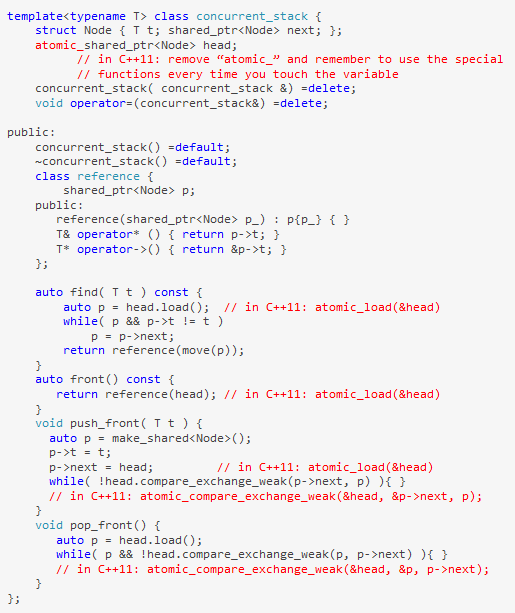
\includegraphics[width=0.8\textwidth]{content/3/chapter6/images/11.png} \\
The expected result with std::atomic\_ref
\end{center}

All changes that are required to compile the program with a C++11 compiler are marked in red. The implementation with atomic smart pointers is a lot easier and hence less error-prone. C++20’s type system does not permit using a non-atomic operation on an atomic smart pointer.

The proposal \href{http://wg21.link/n4162}{N4162} proposed the new types std::atomic\_shared\_ptr and std::atomic\_weak\_ptr as atomic smart pointers. By merging them in the mainline ISO C++ standard, they became partial template specialization of std::atomic, namely std::atomic<std::shared\_ptr<T>{}>, and std::atomic<std::weak\_ptr<T>{}>.

Consequently, the atomic operations for std::shared\_ptr are deprecated with C++20.

\subsubsubsection{6.2.3\hspace{0.2cm} std::atomic\_flag Extensions}

Before I write about std::atomic\_flag extension in C++20, I want to give a short reminder of std::atomic\_flag in C++11. If you want to read more details, read my post about \href{https://www.modernescpp.com/index.php/the-atomic-flag}{std::atomic\_flag} in C++11.

\hspace*{\fill} \\ %插入空行
\noindent
\textbf{6.2.3.1\hspace{0.2cm}  C++11}

std::atomic\_flag is a kind of atomic boolean. It has clear- and set-state functions. I call the clear state false and the set state true for simplicity. Its clear member function enables you to set its value to false. With the test\_and\_set method, you can set the value to true and return the previous value. ATOMIC\_FLAG\_INIT enables initializing the std::atomic\_flag to false.

std::atomic\_flag has two exciting properties, it is

\begin{itemize}
\item 
the only lock-free atomic.

\item 
the building block for higher thread abstractions.
\end{itemize}

With C++11, there is no member function to ask for the current value of a std::atomic\_flag without changing it. This changes with C++20.

\hspace*{\fill} \\ %插入空行
\noindent
\textbf{6.2.3.2\hspace{0.2cm} C++20 Extensions}

The following table shows the more powerful interface of std::atomic\_flag in C++20.

\begin{center}
All operations of std::atomic\_flag atomicFlag
\end{center}

\begin{table}[H]
\centering
\begin{tabular}{ll}
\textbf{Method}             & \textbf{Description}                                           \\ \hline
atomicFlag.clear()          & Clears the atomic flag.                                        \\
\begin{tabular}[c]{@{}l@{}}atomicFlag.test\_and\_set() \\ atomicFlag.test() (C++20)\end{tabular} &
\begin{tabular}[c]{@{}l@{}}Sets the atomic flag and returns the old value. \\ Returns the value of the flag.\end{tabular} \\
\begin{tabular}[c]{@{}l@{}}atomicFlag.notify\_one() (C++20) \\ atomicFlag.notify\_all (C++20)\end{tabular} &
\begin{tabular}[c]{@{}l@{}}Notifies one thread waiting on the atomic flag.\\ Notifies all threads waiting on the atomic flag.\end{tabular} \\
atomicFlag.wait(bo) (C++20) & Blocks the thread until notified and the atomic value changes.
\end{tabular}
\end{table}

The call atomicFlag.test() returns the atomicFlag value without changing it. Further on, you can use std::atomic\_flag for thread synchronization: atomicFlag.wait(), atomicFlag.notify\_one(), and atomicFlag.notify\_all(). The member functions notify\_one or notify\_all notify one or all of the waiting atomic flags. atomicFlag.wait(bo) needs a boolean bo. The call atomicFlag.wait(bo) blocks until the next notification or spurious wakeup. It checks then if the value of atomicFlag is equal to bo and unblocks if not. The value bo serves as a predicate to protect against spurious wakeups. A spurious wakeup is an erroneous notification.

As compared to C++11, default-construction of a std::atomic\_flag is initialized to false state.

The remaining more powerful atomics can provide their functionality by using a mutex. That is according to the C++ standard. So these atomics have a member function is\_lock\_free to check if the atomic internally uses a mutex. On the popular platforms, I always get the answer false. But you should be aware of that.


\hspace*{\fill} \\ %插入空行
\noindent
\textbf{6.2.3.3\hspace{0.2cm} One Time Synchronization of Threads}

Sender-receiver workflows are quite common for threads. In such a workflow, the receiver is waiting for the sender’s notification before Future continues to work. There are various ways to implement these workflows. With C++11, you can use condition variables or promise/future pairs; with C++20, you can use std::atomic\_flag. Each way has its pros and cons. Consequently, I want to compare them. I assume you don’t know the details of condition variables or promises and futures. Therefore, I provide a short refresher.

\hspace*{\fill} \\ %插入空行
\noindent
\textbf{6.2.3.3.1\hspace{0.2cm} Condition Variables}

A condition variable can fulfill the role of a sender or a receiver. As a sender, it can notify one or more receivers.

\hspace*{\fill} \\ %插入空行
\noindent
Thread synchronization with condition variables
\begin{lstlisting}[style=styleCXX]
// threadSynchronizationConditionVariable.cpp

#include <iostream>
#include <condition_variable>
#include <mutex>
#include <thread>
#include <vector>

std::mutex mut;
std::condition_variable condVar;

std::vector<int> myVec{};

void prepareWork() {

	{
	std::lock_guard<std::mutex> lck(mut);
	myVec.insert(myVec.end(), {0, 1, 0, 3});
	}
	std::cout << "Sender: Data prepared." << '\n';
	condVar.notify_one();
}

void completeWork() {

	std::cout << "Waiter: Waiting for data." << '\n';
	std::unique_lock<std::mutex> lck(mut);
	condVar.wait(lck, []{ return not myVec.empty(); });
	myVec[2] = 2;
	std::cout << "Waiter: Complete the work." << '\n';
	for (auto i: myVec) std::cout << i << " ";
	std::cout << '\n';

}

int main() {

	std::cout << '\n';
	
	std::thread t1(prepareWork);
	std::thread t2(completeWork);
	
	t1.join();
	t2.join();
	
	std::cout << '\n';

}
\end{lstlisting}

The program has two child threads: t1 and t2. They get their payload prepareWork and completeWork in lines 40 and 41. The function prepareWork (line 14) notifies that it is done with the preparation of the work: condVar.notify\_one(). While holding the lock, thread t2 is waiting for its notification: condVar.wait(lck, []\{ return not myVec.empty(); \}). The waiting thread always performs the same steps. When awoken, it checks the predicate while holding the lock ([]\{ return not myVec.empty();). If the predicate does not hold, it puts itself back to sleep. If the predicate holds, it continues with its work. In the concrete workflow, the sending thread puts the initial values into the std::vector (line 18), which the receiving thread completes (line 29).

\begin{center}
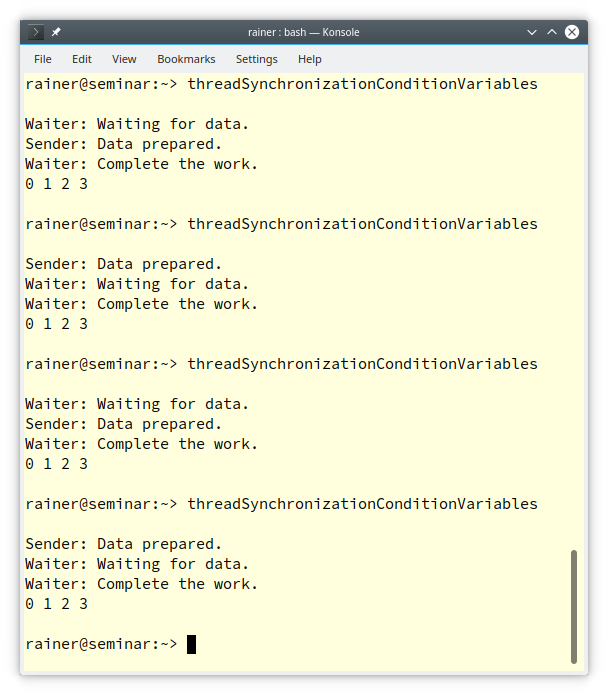
\includegraphics[width=0.8\textwidth]{content/3/chapter6/images/12.png}\\
Thread synchronization with condition variables
\end{center}

Condition variables have many inherent issues. For example, the receiver could be awakened without notification or could lose the notification. The first issue is known as spurious wakeup and the second as lost wakeup. The predicate protects against both flaws. The notification could be lost when the sender sends its notification before the receiver is in the wait state and does not use a predicate. Consequently, the receiver waits for something that never happens. This is a deadlock. When you study the output of the program, you see that every second run would cause a deadlock if I did not use a predicate. Of course, it is possible to use condition variables without a predicate.

If you want to know the details of the sender-receiver workflow and the traps of condition variables, read my posts \href{https://www.modernescpp.com/index.php/c-core-guidelines-be-aware-of-the-traps-of-condition-variables}{“C++ Core Guidelines: Be Aware of the Traps of Condition Variables”}.

Let me implement the same workflow using a future/promise pair.

\hspace*{\fill} \\ %插入空行
\noindent
\textbf{6.2.3.3.2\hspace{0.2cm} Futures and Promises}

A promise can send a value, an exception, or a notification to its associated future. Here is the corresponding workflow using a promise and a future.

\hspace*{\fill} \\ %插入空行
\noindent
Thread synchronization with a promise/future pair
\begin{lstlisting}[style=styleCXX]
// threadSynchronizationPromiseFuture.cpp

#include <iostream>
#include <future>
#include <thread>
#include <vector>

std::vector<int> myVec{};

void prepareWork(std::promise<void> prom) {
	
	myVec.insert(myVec.end(), {0, 1, 0, 3});
	std::cout << "Sender: Data prepared." << '\n';
	prom.set_value();

}

void completeWork(std::future<void> fut){

	std::cout << "Waiter: Waiting for data." << '\n';
	fut.wait();
	myVec[2] = 2;
	std::cout << "Waiter: Complete the work." << '\n';
	for (auto i: myVec) std::cout << i << " ";
	std::cout << '\n';

}

int main() {

	std::cout << '\n';
	
	std::promise<void> sendNotification;
	auto waitForNotification = sendNotification.get_future();
	
	std::thread t1(prepareWork, std::move(sendNotification));
	std::thread t2(completeWork, std::move(waitForNotification));
	t1.join();
	t2.join();
	
	std::cout << '\n';

}
\end{lstlisting}

When you study the workflow, you recognize that the synchronization is reduced to its essential parts: prom.set\_value() (line 14) and fut.wait() (line 21). I skip the screenshot to this run because it is essentially the same as the previous run with condition variables.

Here is more information on promises and futures, often just called \href{https://www.modernescpp.com/index.php/tag/tasks}{tasks}.

\hspace*{\fill} \\ %插入空行
\noindent
\textbf{6.2.3.3.3\hspace{0.2cm} std::atomic\_flag}

Now, I jump directly from C++11 to C++20.

\hspace*{\fill} \\ %插入空行
\noindent
Thread synchronization with a std::atomic\_flag
\begin{lstlisting}[style=styleCXX]
// threadSynchronizationAtomicFlag.cpp

#include <atomic>
#include <iostream>
#include <thread>
#include <vector>

std::vector<int> myVec{};

std::atomic_flag atomicFlag{};

void prepareWork() {

	myVec.insert(myVec.end(), {0, 1, 0, 3});
	std::cout << "Sender: Data prepared." << '\n';
	atomicFlag.test_and_set();
	atomicFlag.notify_one();

}

void completeWork() {

	std::cout << "Waiter: Waiting for data." << '\n';
	atomicFlag.wait(false);
	myVec[2] = 2;
	std::cout << "Waiter: Complete the work." << '\n';
	for (auto i: myVec) std::cout << i << " ";
	std::cout << '\n';

}

int main() {

	std::cout << '\n';
	
	std::thread t1(prepareWork);
	std::thread t2(completeWork);
	
	t1.join();
	t2.join();
	
	std::cout << '\n';

}
\end{lstlisting}

The thread preparing the work (line 16) sets the atomicFlag to true and sends the notification. The thread completing the work waits for the notification. It is only unblocked if atomicFlag is equal to true.

Here are a few runs of the program with the Microsoft Compiler.

\begin{center}
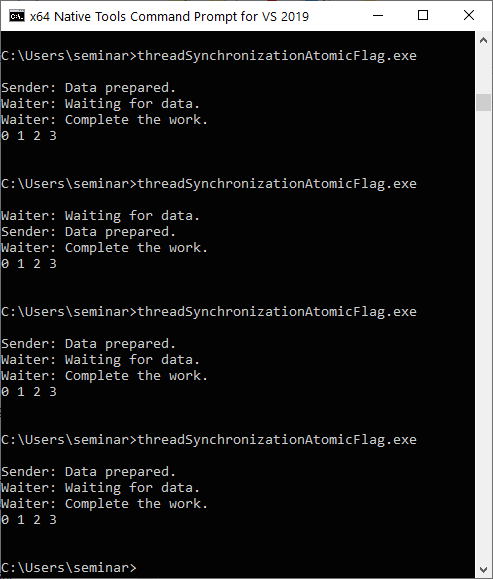
\includegraphics[width=0.8\textwidth]{content/3/chapter6/images/13.png}\\
Thread synchronization with std::atomic\_flag
\end{center}

\subsubsubsection{6.2.4\hspace{0.2cm} std::atomic Extensions}

In C++20, std::atomic. like \href{https://en.cppreference.com/w/cpp/atomic/atomic}{std::atomic\_ref, std::atomic} can be instantiated with floating-point types such as float, double, and long double. In addition, std::atomic\_flag and std::atomic can be used for thread synchronization via the member functions notify\_one, notify\_all, and wait. Notifying and waiting is available on all partial and full specializations of std::atomic (bools, integrals, floats and pointers) and std::atomic\_ref.

Thanks to atomic<bool>, the previous program threadSynchronizationAtomicFlag.cpp can directly be reimplemented.

\hspace*{\fill} \\ %插入空行
\noindent
Thread synchronization with std::atomic<bool>
\begin{lstlisting}[style=styleCXX]
// threadSynchronizationAtomicBool.cpp

#include <atomic>
#include <iostream>
#include <thread>
#include <vector>

std::vector<int> myVec{};

std::atomic<bool> atomicBool{false};

void prepareWork() {

	myVec.insert(myVec.end(), {0, 1, 0, 3});
	std::cout << "Sender: Data prepared." << '\n';
	atomicBool.store(true);
	atomicBool.notify_one();

}

void completeWork() {

	std::cout << "Waiter: Waiting for data." << '\n';
	atomicBool.wait(false);
	myVec[2] = 2;
	std::cout << "Waiter: Complete the work." << '\n';
	for (auto i: myVec) std::cout << i << " ";
	std::cout << '\n';

}

int main() {

	std::cout << '\n';
	
	std::thread t1(prepareWork);
	std::thread t2(completeWork);
	
	t1.join();
	t2.join();
	
	std::cout << '\n';

}
\end{lstlisting}

The call atomicBool.wait(false) blocks if atomicBool == false holds. Consequently, the call atomicBool.store(true) (line 16) sets atomicBool to true and sends its notification.

As before, here are four runs with the Microsoft Compiler.

\begin{center}
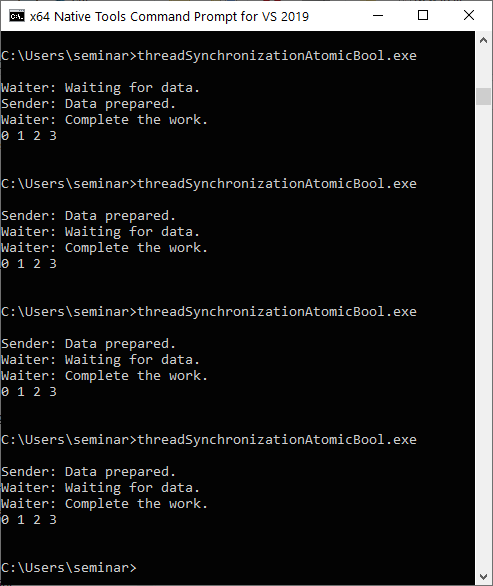
\includegraphics[width=0.8\textwidth]{content/3/chapter6/images/14.png}\\
Thread synchronization with std::atomic<bool>
\end{center}

\begin{tcolorbox}[breakable,enhanced jigsaw,colback=blue!5!white,colframe=blue!75!black,title={Condition Variables versus Promise/Future Pairs versus std::atomic\_flag}]
	
When you only need a one-time notification, such as in the previous program threadSynchronizationConditionVariable.cpp, promises and futures are a better choice than condition variables. Promises and futures cannot be victims of spurious or lost wakeups.
Furthermore, there is neither a need to use locks or mutexes, nor is there a need to use a predicate to protect against spurious or lost wakeups. There is only one downside to using promises and futures: they can only be used once.


I’m not sure if I would use a future/promise pair or atomics such as std::atomic\_flag or std::atomic<bool> for such a simple thread-synchronization workflow. All of them are thread-safe by design and require no protection mechanism so far. Promises and futures are easier to use and atomics are probably faster. I’m only sure that I would not use a condition variable if possible.
	
\end{tcolorbox}


\begin{tcolorbox}[breakable,enhanced jigsaw,colback=mygreen!5!white,colframe=mygreen!75!black,title={Distilled Information}]
	
\begin{itemize}
\item 
std::atomic\_ref applies atomic operations to the referenced object. Concurrent writing and reading is atomic for referenced objects, with no data race. The lifetime of the referenced object must exceed the lifetime of the std::atomic\_ref.

\item 
A std::shared\_ptr consists of a control block and its resource. The control block is thread-safe, but the access to the resource is not. With C++20, we have an atomic shared pointer: std::atomic<std::shared\_ptr<T>{}>, and std::atomic<std::weak\_ptr<T>{}>.

\item 
std::atomic\_flag as a kind of atomic boolean is the only guaranteed lock-free data structure in C++. Its limited interface is extended in C++20. You can return its value, and you can use it for thread synchronization.

\item 
std::atomic, introduced in C++11, gets various improvements in C++20. You can specialize a std::atomic for a floating-point value, and you can use it for thread synchronization.
\end{itemize}
	
\end{tcolorbox}










